\section{Introduction}

This project is really interesting.
I think Stephen Wolfram is the smartest person ever to have stepped
foot on the earth.
When I grow up I want to work for Wolfram Research.
Cellular Automata are everywhere; just look around and you can see
them.
Even the carpeting in Bostock Library is an elementary cellular
autamaton.
Rule 122 with alternating black and white sites for initial
conditions.
See the awesome Figure~\ref{110_map}.

Something about nonlinear dynamics in general and how discrete
nonlinear systems can display complexity with a small number of
parameters--e.g. logistic map.

An Elementary Cellular Autamaton (ECA) is defined in Stephen Wolfram's
\emph{A New Kind of Science}~\cite{anks}

- Rules and rule numbering

- Examples (many figures)

\begin{figure}
\centering
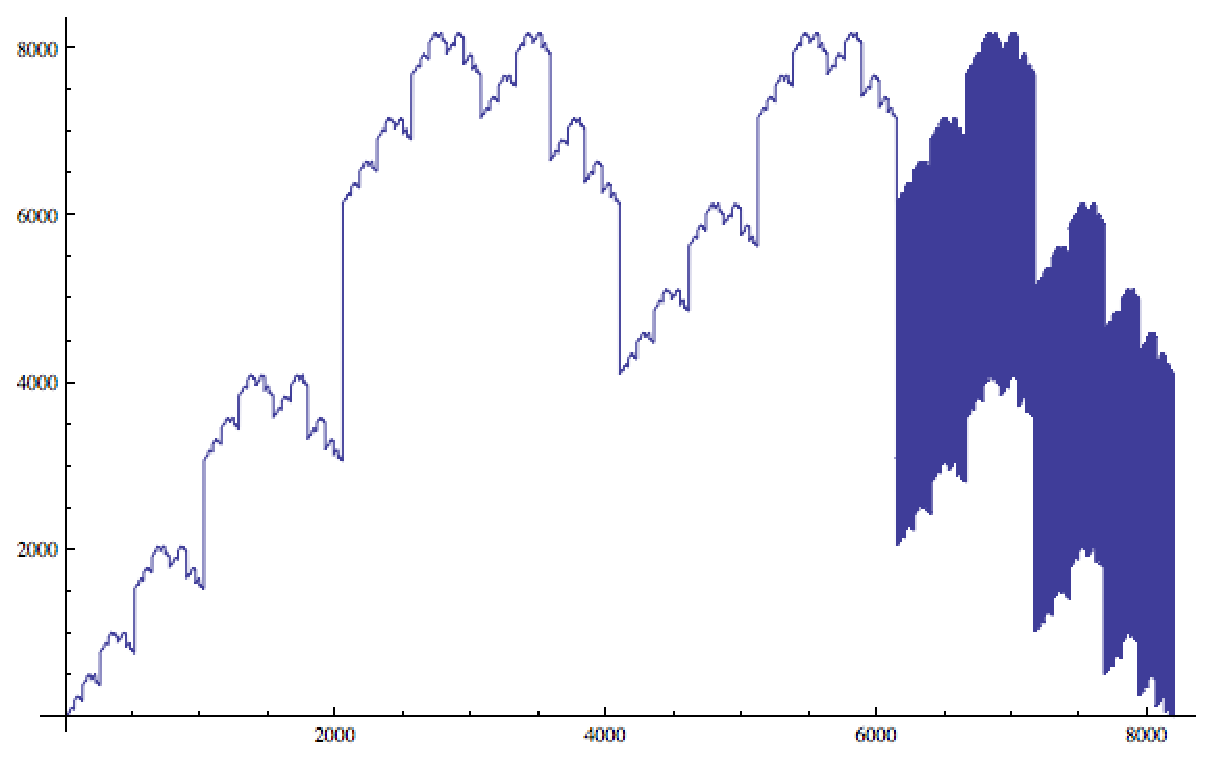
\includegraphics[width=0.49\textwidth]{110_13.eps}
\caption{\label{110_map} Fractal map for rule 110 and a 13-site grid.}
\end{figure}
